%
% 
\subparagraph{Work Package 3 - Access to RIs for Accelerators} \mbox{}
\label{sec:wp3_scientific_output}
% \todo{Scientific output of WP.}


The scientific projects conducted by the WP3 TA users span a wide range of research frontiers, benefiting from the unique capabilities of the facilities. Some highlights are presented below.

\textbf{\textit{Laboratory Astrophysics}} \mbox{}

The \textbf{HRMT-62} and \textbf{HRMT-64} series of experiments, conducted during P2 at the HiRadMat Facility at CERN, focuses on pioneering and high-quality R\&D utilizing the unique characteristics of the facility to conduct laboratory experiments for astroparticle research. The HRMT-62 experiment inaugurated and demonstrated the use of the HiRadMat facility to produce high-intensity, high-density, ultra-relativistic, quasi-neutral electron-positron pair beams, thereby opening up the possibility of studying the microphysics of such pair plasmas through experimental means.
In the subsequent HRMT-64 experiment, with an improved setup that included a secondary target and a magnetic collimating system, the focus was on studying the emergence of magnetic fields associated with the growth of filamentation instabilities. This was done by observing the propagation of collimated relativistic pair-plasma beams through ambient plasma, an analogue for the propagation of astrophysical pair jets through the intergalactic medium.

The results of the experiments were published in well known scientific journals with high impact, triggering the attention of hte community. Up to-date, 5 peer-reviewed articles have been written, 3 of them published in or submitted to Nature, all citing the EURO-LAB support. In total, 14 press releases have been done by the collaborating institutes, including 2 from CERN (bulletin \& courrier). It worth noting that the articles have a high ``attention score'', of 260: 99th percentile of the 329,972 tracked articles of a similar age in all journals. The key scientific result from HRMT-64, only made possible with the EURO-LABS support, was the first-time measurement of the magnetic fields produced by plasma instabilities using a Faraday rotation, seen in Figure~\ref{fig:hiradmat_mag_field_plasma}.
\begin{figure}[H]
    \centering
    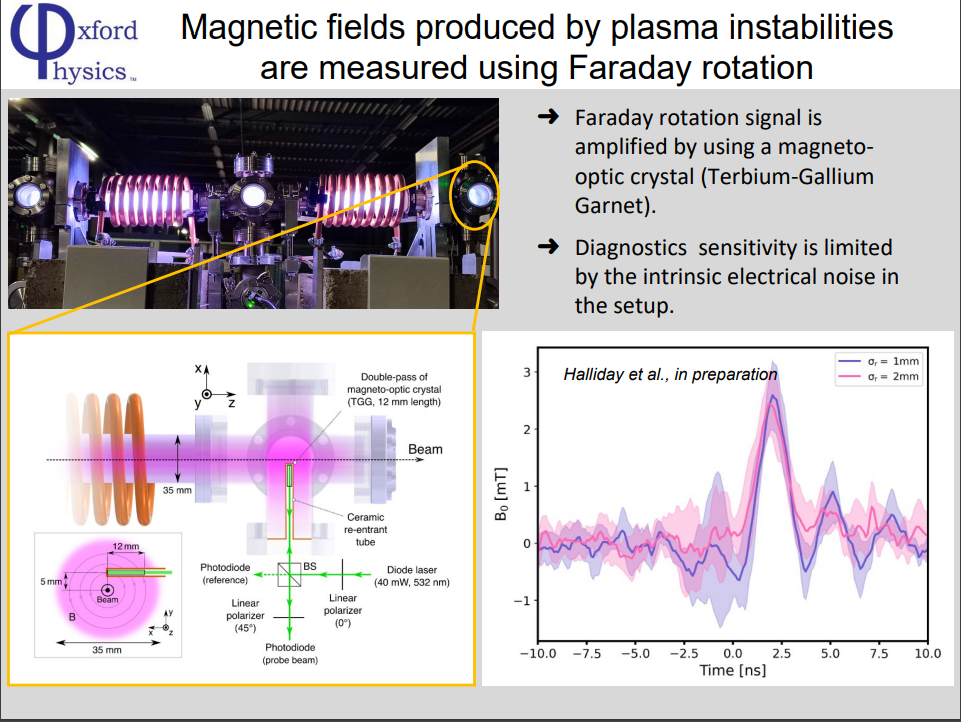
\includegraphics[width=0.75\linewidth]{graphics/HRMT_64_magnetic_field.png}
    \caption{HRMT-64, with the EURO-LABS support measured for first time the magnetic fields produced by plasma instabilities using a faraday rotation in HiRadMat. Courtesy: Prof. G. Gregori, Univ. of Oxford.}
    \label{fig:hiradmat_mag_field_plasma}
\end{figure}

\textbf{\textit{Material R\&D}} \mbox{}

\textbf{HRMT-66} was a novel experiment that pushed forward our current knowledge of material limits, particularly for the often used Glassy Carbon and Beryllium, along with a first-time irradiation of Si$_{3}$N$_{4}$ in order to investigate its exact damage threshold. This is very important for the cooling section of a future muon collider. A photo from the results is shown in Figure~\ref{fig:hiradmat_Si3N4} for Si$_{3}$N$_{4}$ and in Figure~\ref{fig:hiradmat_GC} for Glassy Carbon. The support of EURO-LABS was extremely important since FLUKA simulations were absolutely necessary for the evaluation of the damage mechanisms and precence at CERN was vital for some of the collaborators of the experiment.

\begin{figure}[!h]
    \centering
    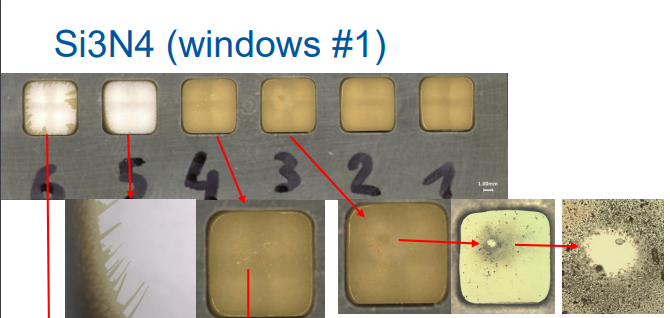
\includegraphics[width=0.85\linewidth]{graphics/hiradmat_si3n4.png} \\
    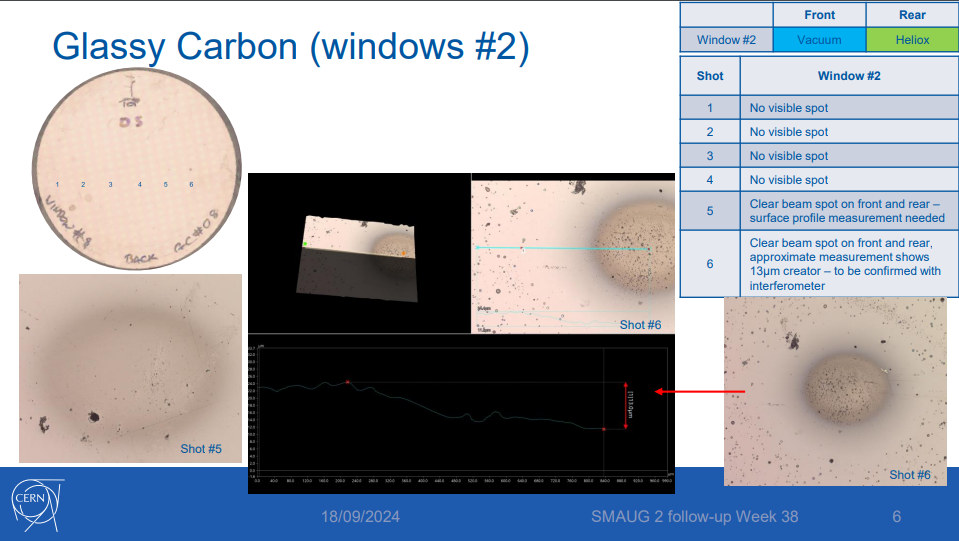
\includegraphics[width=0.85\linewidth]{graphics/hiradmat_GC.png}

    \caption{Top : Beam impact on Si3N4 windows during HRMT-66 experiment. The clear beam spot can be seen in shot \#6 including a small crater. Bottom : Results from HRMT-66 experiment on Glassy Carbon. . (Courtesy: A. Harrison, CERN)}
    \label{fig:hiradmat_Si3N4}
\end{figure}


\textbf{\textit{Instrumentation R\&D}} \mbox{}
\textbf{HRMT-55} is a collaboration between CERN and ESS, to develop a new generation of ionization chambers able to work in high intensify environments, of interest for both Organizations.

Figure~~\ref{fig:hiradmat_IC_response} shows the response of different ionisation chambers (IC) tested for increasing beam intensity. The results indicate a close-to-linear detector performance for all , however with large variations in slope between them. 
\begin{figure}[!h]
    \centering
    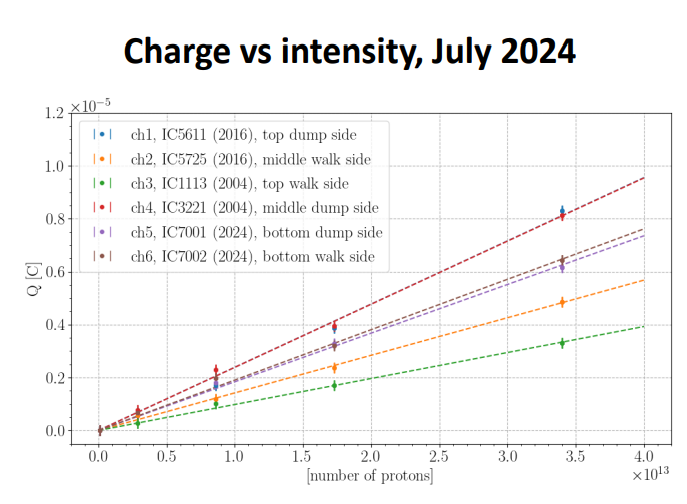
\includegraphics[width=0.8\linewidth]{graphics/hiradmat_IC_response.png}
    \caption{Response (C) of the different ionization chambers tested in HRMT-55. The difference in the slope needs to be understood in detail in a follow-up experiment (HRMT-71) planned for 2025. (Courtesy. S. Grishin, ESS)}
    \label{fig:hiradmat_IC_response}
\end{figure}
This is, for the moment, a puzzling result; therefore, a follow-up experiment \textbf{HRMT-71} is planned for 2025 to further investigate the underlying reasons.

\textbf{R\&D for future accelerators - I}
\todo{PIP-II cavities in SUPRATECH-MACHAFILM}

\textbf{\textit{R\&D for future accelerators}} \mbox{}

Particle accelerators and colliders must cope with a large amount of synchrotron radiation (SR) power being deposited on the vacuum chamber walls.
Photo-stimulated desorption (PSD) leads to increasing pressure and high heat load and is therefore to be investigated using new types of a number of beam screen and vacuum chamber prototypes. The results of this study will be critical for the design of future high-energy hadron colliders such as FCC-hh, in addition this research has potential implications also for the near future of the LHC. 
\begin{figure}[H]
  \centering
  \begin{minipage}[c]{0.45\textwidth}
    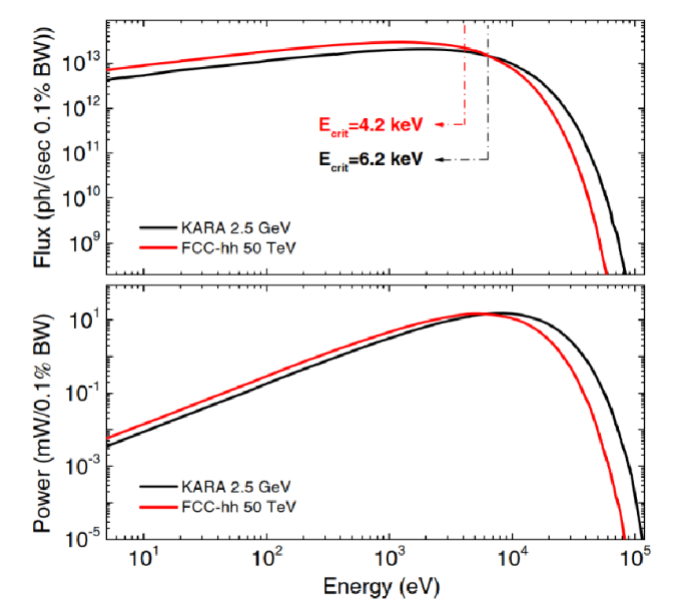
\includegraphics[width=\textwidth]{graphics/wp3-KIT_FCCphotons.png}
  \end{minipage}%
  \hfill
  \begin{minipage}[c]{0.5\textwidth}
    \vspace*{\fill}
    \captionof{figure}{Comparison of the photon flux (top) and power (below) of the FCC-hh at \SI{50}{TeV} proton beam energy in comparison with KARA's at its nominal \SI{2.5}{GeV} electron energy for user %operation. Calculations were performed with SYNRAD+~\footnote{see: L. A. González et al. DOI: 10.1103/Phys.Rev.Accel.Beams 22, 083201, and L. A. González et al. (2021) Phys.Rev.Accel.Beams 24, 113201}
    }
    \label{fig:yourlabel}
    \vspace*{\fill}
  \end{minipage}
\end{figure}

During the EU-project EuroCirCol CERN and KIT realized the BESTEX beamline of CERN at the KIT light source. The storage ring of the KIT light Source is the synchrotron KARA delivering similar spectra as expected at the FCC.

CERN installed a residual gas analyser in the central part of the BESTEX test chamber  before the start of the FCC beam screen prototype experiment (no.5, with saw-tooth profile to decrease synchrotron radiation photon scattering) in period P1 (EURO-LABS-KIT-KARA-2023-01). In period P2 this prototype was exchanged by the new beam-screen prototype no. 6 with amorphous carbon coating (aC). aC is a stable and inert material, deposited via sputtering techniques onto the internal wall of a circular tube (carried out at CERN).  The main feature of aC is its extremely low secondary electron yield, which is necessary to avoid electron cloud instability in accelerators with positively charged beams. In the long-term experiment at KARA (EURO-LABS-KIT-KARA-2023-03), the beam-screen prototype no. 6 was irradiated at a flat angle of incidence and cooled with LN2. The increase in pressure was measured. In addition, the composition of the species outgassing from the beam screen was determined at CERN's BESTEX beamline at KARA. The experiment began installation in August 2023 and the prototype was irradiated with over 480 KARA synchrotron light until the first quarter of 2024. The prototype is still installed in BESTEX and is waiting to be exchanged for the next one, which is currently being prepared
\begin{figure}[!h]
    \centering
    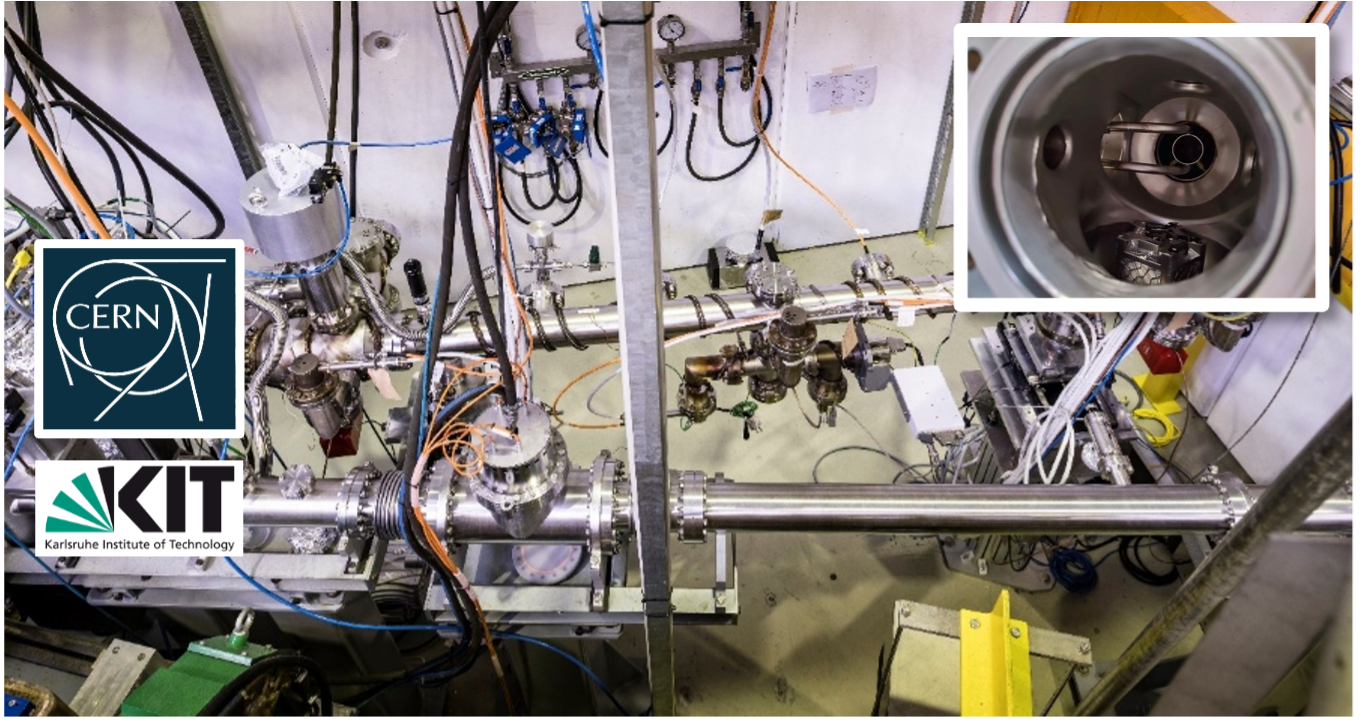
\includegraphics[width=0.75\linewidth]{graphics/wp3-KIT_BESTEX.png}
    \caption{CERN installed the BESTEX beamline at KARA since 2019 (EU project EuroCirCol). BESTEX was used for up to now two actual TA experiments within EURO-LABS. A goal is the exploration of the vacuum performance of the FCC-hh beam screen to protect the cold superconducting magnets from the 
direct irradiation high-power SR photon beams.
}    
    \label{fig:kit_bestex}
\end{figure}

The KARA experiment (EURO-LABS-KIT-KARA-2023-04) of the University Lille aimed to observe, understand and control the ultrafast self-organisation of relativistic electron bunches in accelerator facilities. A central goal is to master the emission of giant terahertz (THz) pulses in coherent synchrotron radiation (CSR), which is a proposal for new THz sources. Another important goal was the improvement of novel ultrafast observation instruments. KARA is one of the only electron storage rings in the world where the shape of relativistic electron bunches can be directly ‘studied’ in a storage ring facility. The techniques of chaos control (feedback control of periodic orbits) for achieving stable THz-CSR emissions, which the team at the University of Lille had already successfully tested at the SOLEIL synchrotron, were transferred to the KIT light source KARA, and the results have thus been compared between the machines and with theory. At KARA, the opportunity was taken to observe the development of the longitudinal bunch profile in real time with the help of the existing electro-optical near-field setup. In this experiment, an advanced control loop from chaos control theory was implemented on a fast FPGA board to control the amplitude of one of the two main radiofrequency (RF) cavities in the electron storage ring KARA at KIT. The CSR emission of THz power at high level was stabilised to control the micro-bunching instability. The fast Schottky diodes in the KIT-IR2 beamline at KARA were used and the THz power was measured in real time with the high-speed data acquisition card KAPTURE developed by KIT.
\begin{figure}[H]
    \centering
    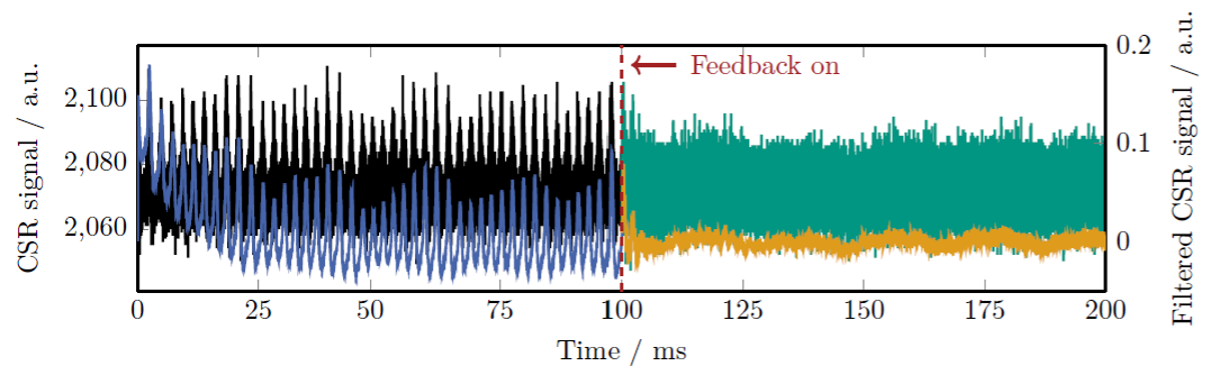
\includegraphics[width=0.75\linewidth]{graphics/wp3-KIT_CSRsignal.png}
    \caption{The CSR signal was measured with a fast Schottky diode (at a KIT infrared beam line). After \SI{100}{ms} the team of the University Lille (F) switched on the FPGA-based feedback loop. For better visibility, the raw signal (black, left \& green, right) was filtered (blue, left \& orange, right) to remove the fast sinusoidal fluctuation. Suppression of the sawtooth outburst fluctuation variance by a factor of 28 in the CSR emission at the KARA electron storage ring, after switching on the FPGA-based feedback loop developed by the PhLAM team of University Lille. The fast CSR fluctuations are still present after the feedback is switched on, leading to a stabilization of the THz emission. Publication in preparation.}    
    \label{fig:kit_csr}
\end{figure}

FCC-ee precision physics measurements require an accurate and precise determination of the centre-of-mass collision energy, which can be obtained from the beam energies. Since the depolarisation frequency is directly proportional to the beam energy, a promising way to determine this energy is to depolarise transversely polarised packets. This resonant depolarisation (RDP) has long been used in KARA whereby the resonance frequency is measured via the change in the Touschek lifetime. At KARA, a first RDP measurement campaign (EURO-LABS-KIT-KARA-2023-05) with numerous scan settings and bundle configurations was carried out to investigate how this technique could be applied at FCC-ee, in particular the sensitivity to parameters such as the scan speed of the depolariser and the scan velocity. The measurement campaign was successful and the users at CERN expressed interest in carrying out another measurement campaign at a later target point.
\begin{figure}[H]
    \centering
    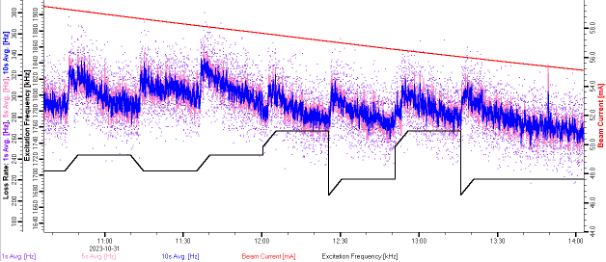
\includegraphics[width=0.75\linewidth]{graphics/wp3-KIT_RDPscans.png}
    \caption{More than 40 successful RDP scans were realized at KARA by scanning direction up and down for scanning times of \SI{100}{s} to \SI{600}{s}, respectively}    
    \label{fig:kit_rdp}
\end{figure}

RDP results published in:
\begin{itemize}
\item FCCIS WP2-workshop, 2023-11-15, B. Härer et al.: Polarisation studies at KARA
\item and in the following IPAC papers: \\ https://doi.org/10.18429/JACoW-IPAC2024-TUPG33, \\ https://doi.org/10.18429/JACoW-IPAC2024-WEPG51, and \\ https://doi.org/10.18429/JACoW-IPAC2024-WEPR20
\end{itemize}

Bunch-by-bunch (BBB) feedback systems are essential for the realisation of ultra-low emittance rings that allow electron beams to reach high-quality states for use in synchrotron radiation light sources and colliders. Following the workshop WP7.2 of the EU project I.FAST on BBB feedback systems, which was attended by more than 40 experts on BBB systems from all over the world, the following three experiments were carried out at the request of the experts in connection with the BBB systems carried out at the KARA storage ring and at the booster synchrotron with real electron beams by operating the BBB systems installed in each of the two accelerators(EURO-LABS-KIT-KARA-2024-06). The aim of the first experiment at KARA was to manipulate the vertical beam size by exciting the betatron oscillation with the BBB system to improve the Touschek beam lifetime. The goal of this experiment was to look for common procedures for commissioning bunch-by-bunch feedback systems. The goal of the third experiment was to longitudinal kicks with the bunch-by-bunch feedback system and the stripline kicker installed in the booster synchrotron. This experiment will lead to the next step, such as longitudinal manipulation of beams to improve booster beam quality. Data and results of the three experimental topics have been shared with all interested participants, and the data analysis and subsequent discussions are ongoing. 


According to the design of the FCC, the desired mechanical alignment tolerances of the magnets are in the range of \SI{100}{\micro\meter} to \SI{150}{\micro\meter}. However, to achieve the ambitious research goals at the FCC, a low (10-20 µm) relative alignment of the quadrupoles and sextupoles is required. For this purpose, correction magnets are provided to steer the beam in the direction of the magnetic centre, which is known as beam-based alignment (BBA). The BBA must be performed for approx. 1870 quadrupoles and approx. 630 sextupoles, so in addition to the accuracy, the average time required to determine the individual magnetic offset is a key parameter for the selection of the BBA method. The development of a concept for the BBA at FCC-ee is currently based on simulations but is to be supported by proof-of-principle tests on existing machines, for which experiments were carried out at KARA (EURO-LABS-KIT-2024-KARA-07).  Strategies were successfully investigated that will significantly reduce the time required for the BBA at FCC.


\textbf{\textit{Novel detector R\&D}} \mbox{}

\begin{description}
\item[MM\_TCP]: The experiment goal was to test and validate TPC performances of two MicroMegas detectors based on a strip read out system. The resistive Micromegas chambers are frontier Micro-Pattern Gas Detectors with a planar geometry and with an amplification gap of the order of \SI{18}{\micro\meter} between the read-out (RO) PCBs and the mesh. Similar detectors have been widely used and recently installed in the muon spectrometer of one of the LHC experiment, covering a dimension of \SI{2400}{\meter\tothe{2}}.
The purpose of the test beam is to study and tune the DAQ based on APV technology in order to adapt to the acquisition window required for TPC purposes.
\begin{figure}[H]
    \centering
    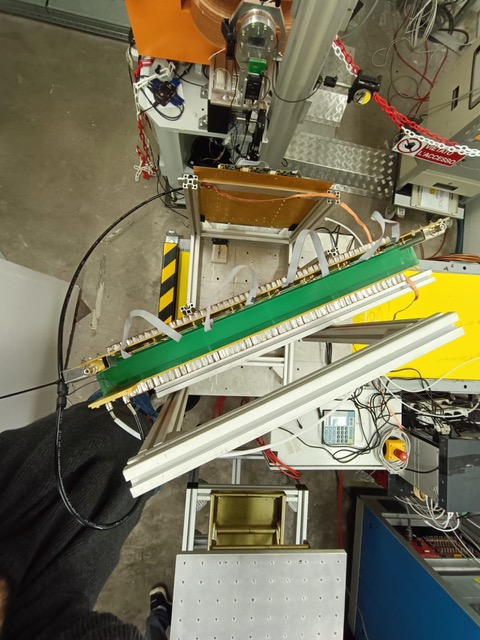
\includegraphics[width=0.48\linewidth]{graphics/BTF-MMTPC2.jpeg}
    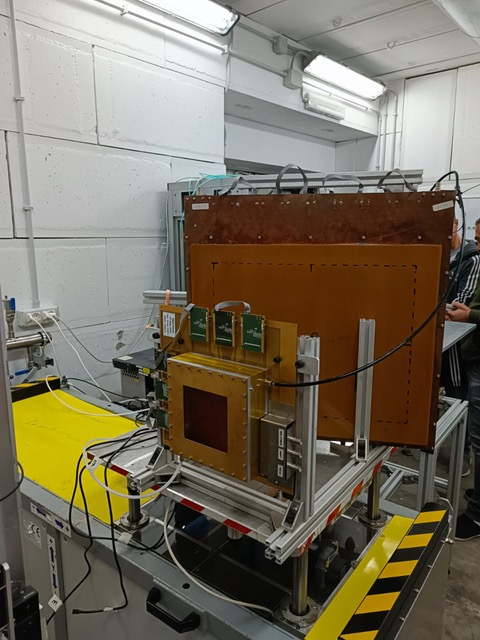
\includegraphics[width=0.48\linewidth]{graphics/BFT-MMTPC3.jpeg}
    \caption{Photo of the experimental setup in the BTF line.}    
    \label{fig:kit_rdp}
\end{figure}
Two different types of Micromegas, one of which never previously tested, have been experimentally characterized. The planned test and some other extra test have been fully acquired, with calibration and load curve in different beam configuration especially for flux and multiplicity.
The experiment resulted to be well-planned, executed smoothly, and achieved its goals. The combination of on-site and remote support, along with continuous monitoring of the system parameters, contributed to the overall success of the operation.
Experiment Duration: 1 week or 168 h (2023, 20-27 November)

\item[MICROGASTRACK]:
The experiment aimed at testing a novel micromegas gas chamber with variable high voltage which could enable both to track the secondary particles produced in the interactions and to measure the initial high intensity beam parameters. The device under test combines the functionalities of micropattern gas detectors for precise sub millimetre tracking and gas detectors for beam monitoring.

The detector that was expected to be ready for the test beam time, was unfortunately not completed in time. However, the team was able to test the MM electronics and integrate with the BTF timing and triggering. Additionally, during the beam time, a successful integration of future detector support was achieved. The team had also the possibility to test the detector electronics (APV25) and the communication with the pre-existing DAQ system
Experiment Duration: 2 weeks or 336 h (2024, 4-18 November)

\item[CALOBEAMPIX]:
The experiment goal was to test silicon pixel detectors for simultaneous measurement of electron/positron beams with two different types of detectors: calorimeter and silicon pixel detector. 

The following experimental goals were reached:
\begin{itemize}
    \item Operate simultaneously Timepix3 array and lead glass calorimer
    \item Develop threshold equalization procedure for the Timepix3 pixels
    \item Synchronized data acquisition (either online or offline) of Timepix3 and lead-glass calorimeter
    \item Calibrate the lead glass block for different beam multiplicity using the Timepix3 data
\end{itemize}
Experiment Duration: 1 week or 168 h (2024, 9-16 December)
\end{description}


%\textbf{Medical Physics R\&D}

%\begin{description}
%    \item[AI1] Artificial Intelligence readiness at CLEAR. Done, Reimbursed (A. Pollastro, 40 units)
%    \item[LUXE2] Done, reimbursed (F. Lasagni-Manghi, 40 units)
%    \item[THz] THz sources on Smith-Purcell radiation, THZ1 > Initial visit + preparation done,  will not be reimbursed (paid by Users Lab) (T. Zhang, 16 units)
%    \item[SE1] Electron collimation at CLEAR (SE1) > Done, to be reimb. (N. Delerue, D. Dauvergne, 64 units)
%\end{description}

\textbf{Applications}


\begin{itemize}
\item One-electron oxidation of S-adenosyl methionine,
\item Crosslinking of self-assembled fatty acids on copper by electron beam irradiation,
\item Effect of ionizing irradiation on dried fruits,
\item Influence of 10 MeV accelerated electrons on structure and properties of sheep wool fibres as a potential component for preparation of polymer-based composite materials
\item Irradiation engineering of biopolymer-based formulation for wound management and targeted drug delivery devices,
\item Bioactivity of irradiated foods by low energy e-beam,
\item Face masks recycling with the use of radiation technologies.
\end{itemize}